\documentclass[twoside,11pt]{article}
\setlength{\oddsidemargin}{0.0 in}
\setlength{\evensidemargin}{-0.0 in}
\setlength{\topmargin}{-0.6 in}
\setlength{\textwidth}{6.5 in}
\setlength{\textheight}{8.5 in}
\setlength{\headsep}{0.15 in}
\setlength{\parindent}{0 in}
\setlength{\parskip}{0.1 in}

%
% ADD PACKAGES here:
%

\usepackage{amsmath,amsfonts,graphicx}
\usepackage{multirow}
\usepackage{comment}
\usepackage[]{algorithm2e}
\usepackage{subfig}

%
% The following commands set up the lecnum (lecture number)
% counter and make various numbering schemes work relative
% to the lecture number.
%
\newcounter{lecnum}
\renewcommand{\thepage}{\arabic{page}}
\renewcommand{\thesection}{\arabic{section}}
\renewcommand{\theequation}{\arabic{equation}}
\renewcommand{\thefigure}{\arabic{figure}}
\renewcommand{\thetable}{\arabic{table}}

%
% The following macro is used to generate the header.
%
\newcommand{\lecture}[4]{
   \pagestyle{myheadings}
   \thispagestyle{plain}
   \newpage
   \setcounter{lecnum}{#1}
   \setcounter{page}{1}
   \noindent
   \begin{center}
   \framebox{
      \vbox{\vspace{2mm}
    \hbox to 6.28in { {\bf 49274: Advanced Robotics
		\hfill Spring 2020} }
       \vspace{4mm}
       \hbox to 6.28in { {\Large \hfill Assignment #2: Path Planning \hfill} }
       \vspace{3mm}
	   \hbox to 6.28in { { #3 \hfill  Due date: \textbf{#4}} }
      \vspace{2mm}}
   }
   \end{center}
   \markboth{Assignment #2}{Assignment #2}
}
%

\begin{document}
\lecture{1}{September 08}{University of Technology Sydney (CAS)}{September 08}

\section*{Introduction}
The basic motion planning algorithms consist of two steps. Path planning and Control. In this
assignment emphasis will be primarily on the first step, where you will be implementing an A*
planner and a waypoint smoothing algorithm.

\section*{Path Planning}
The path planning problem states: Given a starting and ending configurations, how can our robot reach the goal with the lowest “cost”. Simply put, the path planning problem is to find the “cheapest” (e.g., shortest) sequence of actions that will lead our robot from the starting location to the ending location.

\subsection*{Example}
First we simplify our environment into discrete grid cells and we define our starting location (S) and goal location (G). Obstacles are represented by (x). Our robot is only allowed to move in 4 different irections: right, left, up and down. 
\begin{table}[ht]
	\label{tab:map-1}
	\begin{center}
		\begin{tabular}{|c|c|c|c|c|c|c|}
			\hline
			0 & 0 & 0 & 0 & 0 & 0 & 0 \\
			\hline
			0 & 0 & x & x & 0 & 0 & 0 \\
			\hline
			0 & 0 & x & 0 & 0 & 0 & 0 \\
			\hline
			0 & 0 & x & G & 0 & 0 & 0 \\
			\hline
		\end{tabular}
	\end{center}
\end{table}
Visually we can see that the shortest path with lowest cost to reach the goal would be in 11 steps. Given that the cost of each move (\textit{g}) is 1, the total cost is 11.
\begin{table}[ht]
	\label{tab:map-2}
	\begin{center}
		\begin{tabular}{|c|c|c|c|c|c|c|}
			\hline
			3 & 4 & 5 & 6 & 7 & 8 & 9 \\
			\hline
			2 & 3 & x & x & 8 & 9 & 7 \\
			\hline
			1 & 2 & x & 10 & 9 & 10 & 11 \\
			\hline
			0(S) & 1 & x & 11(G) & 10 & 11 & 12 \\
			\hline
		\end{tabular}
	\end{center}
\end{table}
Algorithmically, searching for the goal can be done by a method called Dijkstra’s algorithm. From the starting cell (S) we look in the directions \textbf{top}, \textbf{right}, \textbf{down} and \textbf{left} in any order and increment the cost by 1 every time we expand. To keep track of our frontier nodes (i.e., nodes that can be
expanded from), we use a list called \texttt{openList}. \texttt{openList} is a list of nodes: it consists of a \textit{x}, \textit{y} position and the cost associated with that node.

\texttt{openList}: \textbf{Step 1}
\begin{table}[ht]
	\label{tab:step-1}
	\begin{center}
		\begin{tabular}{|c|c|c|}
			\hline
			\textit{x} & \textit{y} & \texttt{cost} \\
			\hline
			1 & 1 & 0\\
			\hline
		\end{tabular}
	\end{center}
\end{table}
\newline To begin the open list will only consist of the start position. Then we expand:

\texttt{openList}: \textbf{Step 2}
\begin{table}[ht]
	\label{tab:step-2}
	\begin{center}
		\begin{tabular}{|c|c|c|}
			\hline
			\textit{x} & \textit{y} & \texttt{cost} \\
			\hline
			1 & 2 & 1\\
			\hline
			2 & 1 & 1\\
			\hline
		\end{tabular}
	\end{center}
\end{table}

The node that was expanded from is first taken out of our open list, this should be done every time
a new node is expanded from. Next we search and add all the new nodes (i.e., neighbours) to our
open list. A good practice is to check the nodes being expanded from as closed, this means that
when performing new searches, closed nodes will be avoided.

\texttt{openList}: \textbf{Step 3}
\begin{table}[ht]
	\label{tab:step-3}
	\begin{center}
		\begin{tabular}{|c|c|c|}
			\hline
			\textit{x} & \textit{y} & \texttt{cost} \\
			\hline
			2 & 1 & 1\\
			\hline
			2 & 2 & 2\\
			\hline
		\end{tabular}
	\end{center}
\end{table}

It is of utmost importance to always select the node with the lowest cost to expand from, as you
can see the next node above will be $\begin{bmatrix}
\mathbf{2} & \mathbf{1} & \mathbf{1}\end{bmatrix}$.\\
If you continue to do the search until the goal is reached while tracking each expansion, by incrementing a counter by 1, then an expand grid can be obtained.

\subsection*{Expand Grid}
\begin{table}[h!]
	\label{tab:map-3}
	\begin{center}
		\begin{tabular}{|c|c|c|c|c|c|c|}
			\hline
			6 & 7 & 8 & 9 & 10 & 11 & 12 \\
			\hline
			4 & 5 & x & x & 12 & 14 & 16 \\
			\hline
			2 & 3 & x & 19 & 15 & 17 & 20 \\
			\hline
			0(S) & 1 & x & 22(G) & 18 & 21 & 0 \\
			\hline
		\end{tabular}
	\end{center}
\end{table}

From this expand grid, the \textbf{optimum policy} or best path, indicated by *, can be found by tracing
backwards from the goal back to the start. Search by following the lowest expand number.


\subsection*{Optimum Policy}
When searching for the optimum path incrementally, you can see that some search directions will
take you away from the goal. 

\begin{table}[ht]
	\label{tab:map-4}
	\begin{center}
		\begin{tabular}{|c|c|c|c|c|c|c|}
			\hline
			6 & 7* & 8* & 9* & 10* & 11 & 12 \\
			\hline
			4 & 5* & x & x & 12* & 14 & 16 \\
			\hline
			2 & 3* & x & 19 & 15* & 17 & 20 \\
			\hline
			0(S)* & 1* & x & 22(G) & 18* & 21 & 0 \\
			\hline
		\end{tabular}
	\end{center}
\end{table}
This can be considered wasted effort and time consuming especially if the map is complex and large. 
A* search solves this problem by introducing a heuristic cost (h)
to the cost of each step. A simple (admissible) heuristic would be how far away each grid cell is
from the goal, ignoring the obstacles (Manhattan distance).

\subsection*{Heuristic Grid}
\begin{table}[ht]
	\label{tab:h-g}
	\begin{center}
		\begin{tabular}{|c|c|c|c|c|c|c|}
			\hline
			6 & 5 & 4 & 3 & 4 & 5 & 6 \\
			\hline
			5 & 4 & 3 & 2 & 3 & 4 & 5 \\
			\hline
			4 & 3 & 2 & 1 & 2 & 3 & 4 \\
			\hline
			3 & 2 & 1 & 0(G) & 1 & 2 & 3 \\
			\hline
		\end{tabular}
	\end{center}
\end{table}
Now our cost becomes $f(i, j) = g(i, j) + h(i, j)$, where $g(i, j)$ is our original cost and $h(i, j)$ is the new heuristic cost.

\begin{table}[ht]
	\label{tab:map-5}
	\begin{center}
		\begin{tabular}{|c|c|c|c|c|c|c|}
			\hline
			9=(3+6) & 9=(4+5) & 9=(5+4) & 9=(6+3) & 11=(7+4) & 13=(8+5) & 15=(9+6) \\
			\hline
			7=(2+5) & 7=(3+4) & x & x & 11=(8+3) & 13=(9+4) & 15=(9+6) \\
			\hline
			5=(1+4) & 5=(2+3) & x & 11=(10+1) & 11=(9+2) & 13=(10+3) & 15=(11+4) \\
			\hline
			(S) & 3=(1+2) & x & (G) & 11=(10+1) & 13=(11+2) & 15=(12+3) \\
			\hline
		\end{tabular}
	\end{center}
\end{table}

If we only expand to the node with the lowest cost, then the shortest path to the goal can be
found without exhaustively searching. You can see that grids with costs values above 11 are never
expanded from if the above searching method is applied.


\subsection*{Path Smoothing}
Now that we have an optimum path, we want to find the best way the robot can follow. However,
our current path has many disadvantages. For example, the current set of way points would require
our robot to take 90 degree turn, which is impossible for some robots. Another disadvantage is that
the robot would need to stop before making turns resulting in abnormal motion for the robots.
By smoothing all our way-points, the robot motion to its goal location will become much more
fluid and natural. To perform this smoothing we define and then solve an optimization problem.
Suppose ${S_i}$ is the $i − th$ smooth way-point (the ${x}$ and ${y}$ location of the point), and $p_i$ is the $i − th$ point in our original way-points. We want to minimize a \textbf{weighted} sum of:

\begin{enumerate}
  \item (squared) distance between smooth adn original points (i.e., $p_i$ and $s_i$ )
  \item (squared) distance between consecutive smooth points (i.e., $s_i$ and $s_{i+1}$ ).
\end{enumerate}

   \begin{figure*}[t]
   	\centering
   	\subfloat[Original Path ]
   	{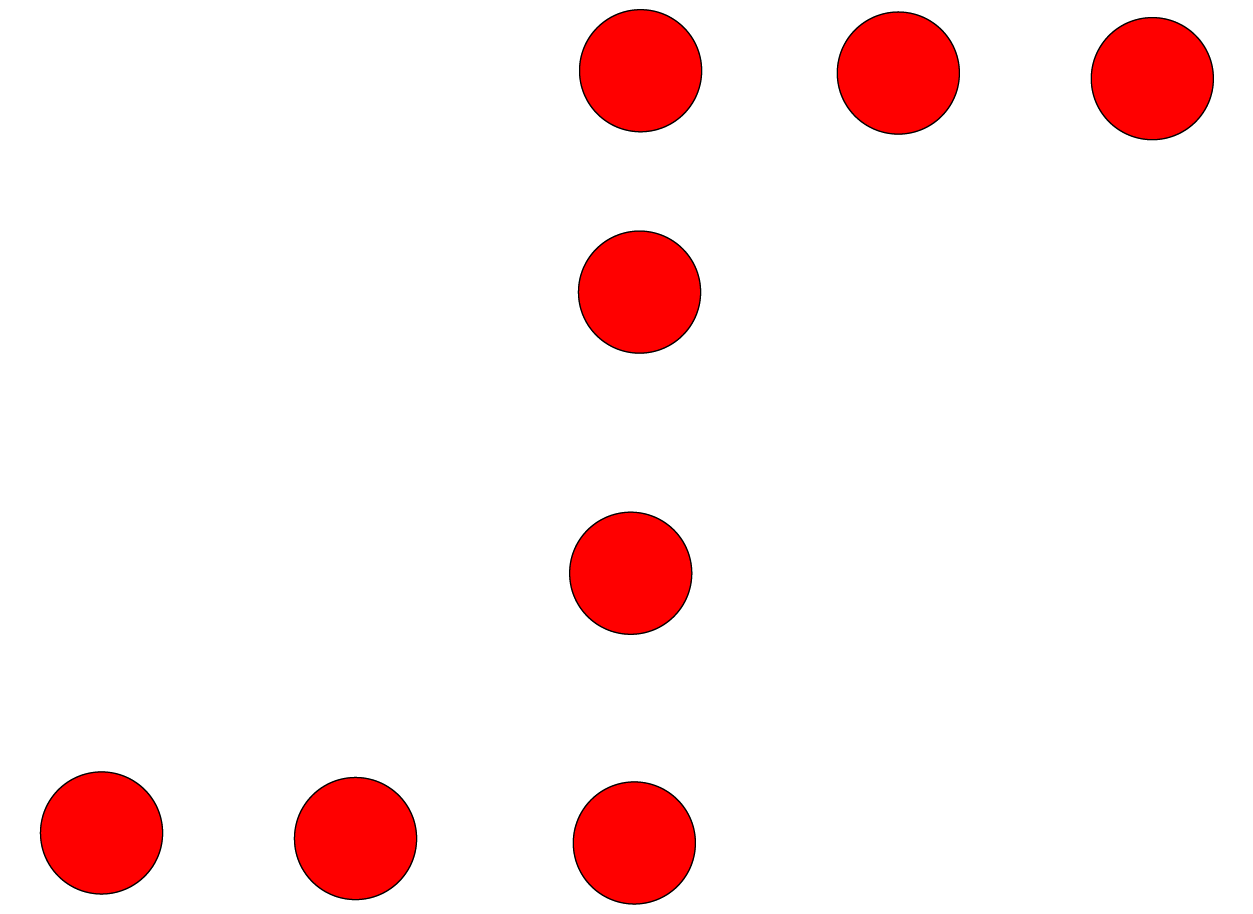
\includegraphics[width=0.40\columnwidth]{./figures/b4-smooth.png}\label{con1}}
   	\subfloat[Smooth Path ]
   	{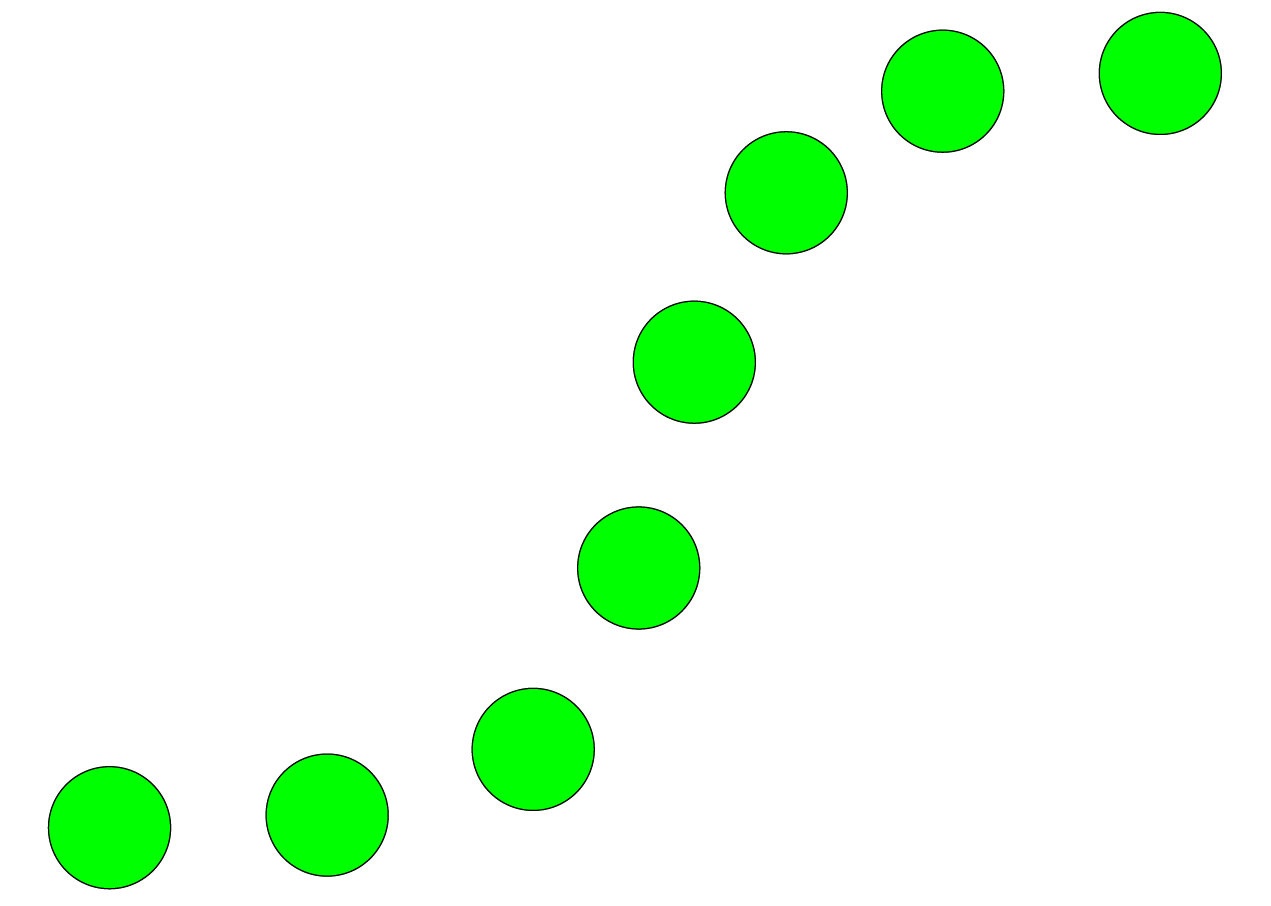
\includegraphics[width=0.40\columnwidth]{./figures/after-smooth.png}\label{con2}}
   	\caption{Path Smoothing}
   	\label{Exam_con}
   \end{figure*}

It is important to realize that, if we only minimize (1) then we will get the original path, and if we
only minimize (2) then we will get the straight line linking the start and goal. Therefore for our
algorithm to work, we must simultaneously minimize both ( a weighted sum of them) and apply
weight $\alpha$ and $\beta$ to each criteria. These values will affect the smoothness of the new path. You need
to tune the values of weights ($\alpha$ and $\beta$).\\*\\*
\begin{center}
\line(1,0){500}
\end{center}



\section*{Compiling and Running in ROS}
\subsection*{Compilation}
Run following commands in a terminal window.
\begin{itemize}
	\item Download \texttt{path\_planner.zip} package, extract the folder \texttt{path\_planner} into
	{$\sim$/catkin\_ws/src/}.
	\item The file structure under \texttt{path\_planner} is shown below
	\item Verify installation successful by running command: \texttt{rospack find path\_planner}
	\item The system should respond with \texttt{$\sim$/catkin\_ws/src/path\_planner}
	\item Change directory:  \texttt{cd $\sim$/catkin\_ws}
	\item Build catkin\_ws: \texttt{catkin build} 
\end{itemize}

\subsection*{Running ROS}
Here a simplified way (one liner) of loading the astar planner package, this is possible in the most
recent download package, it contains a new version of launch file that loads everything in one step.
\begin{itemize}
	\item \texttt{roslaunch astar planner astar planner.launch}
\end{itemize}
Alternatively you may want to load the system step by step, in this case, make sure the last two
lines in the file astar planner.launch are commented out, as in previous version of your download
package.
\begin{itemize}
	\item \texttt{roscore}
	\item \texttt{cd $\sim$/catkin\_ws/src/path\_planner}: to change to the right directory
	\item \texttt{rosrun map\_server map\_server data/map.yaml}
	\item \texttt{rosrun rviz rviz -d data/planner\_conf.rviz}: to start rviz with the configuration file loaded
	\item \texttt{roslaunch path\_planner path\_planner.launch}: to start the planner with certain parameters
\end{itemize}
\begin{figure}[h!]
	\caption{package content}
	\centering
	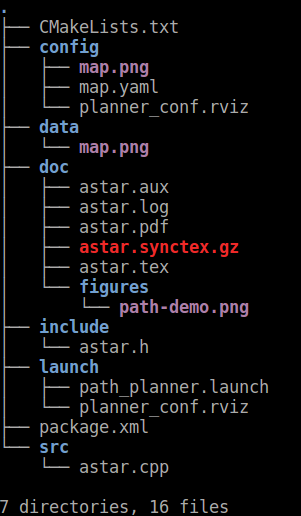
\includegraphics[width=0.3\textwidth]{./figures/file-tree.png}
\end{figure}

\subsubsection*{Parameters}
You are required to change the start position and target position in the launch file when you test
your program. The basic explanation of the launch file is as below:
\begin{itemize}
	\item \textbf{startx} and \textbf{starty} denote the start position in map coordinate system
	\item \textbf{goalx} and \textbf{goaly} denote the goal position in map coordinate system
\end{itemize}

\begin{figure}[h!]
\caption{An example result of A*}
\centering
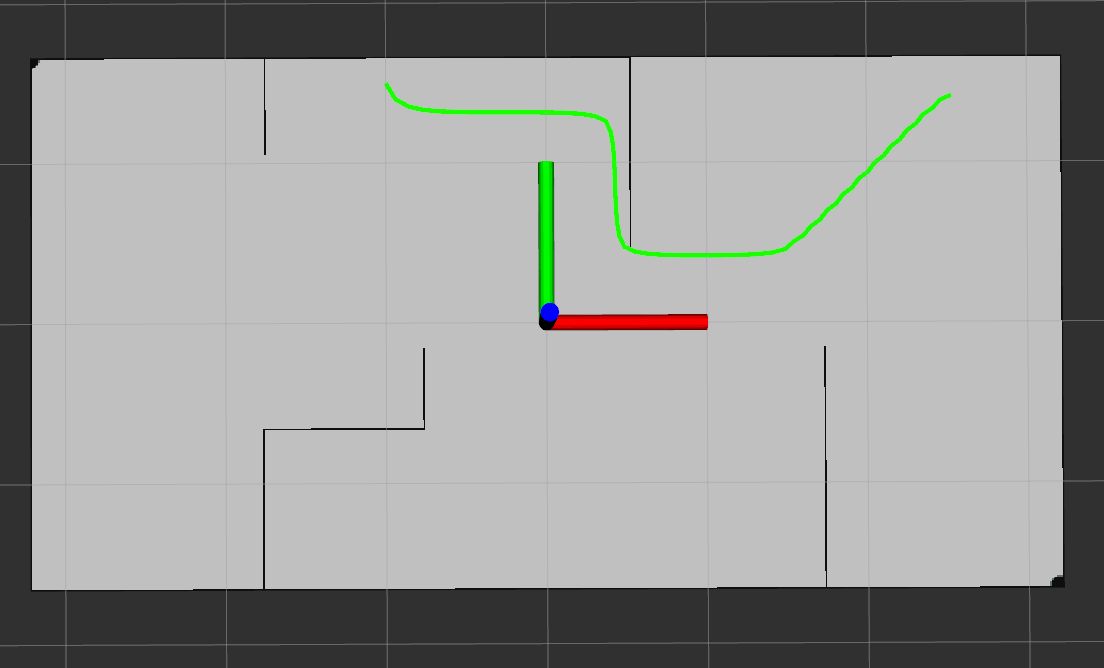
\includegraphics[width=0.7\textwidth]{./figures/path-demo.png}
\end{figure}

\section*{Data Structure in Brief}

Before you begin coding, it is very important to understand some of the functions and structures
given to you in the \texttt{Astar} class.

\subsection*{Variables}
\begin{itemize}
	\item \textbf{Grid}: This structure represents a grid cell, there are four variables that can be used for each
	grid. These variables are all set to 0 initially.
	\begin{itemize}
		\item \texttt{occupied} 
		\item \texttt{closed}
		\item \texttt{expand}
		\item \texttt{heuristic}
	\end{itemize}
	\item \textbf{Node}: A node is represented by an index x position, index y position and a cost value.
	\begin{itemize}
		\item \texttt{x} 
		\item \texttt{y}
		\item \texttt{cost} 
	\end{itemize}
	\item \textbf{Waypoint}: A waypoint is the pose which may belongs to the shortest path.
	\begin{itemize}
		\item \texttt{x}
		\item \texttt{y}
	\end{itemize}
\end{itemize}

\subsection*{Variables}
\textbf{Hint}: If you are still confused with the meanings of the parameters, please read \texttt{astar.h} for detail.
\begin{itemize}
	\item \texttt{gridmap\_} : 2-dimensional grid map, with index rule \texttt{[y][x]}, the related variables are \texttt{grid\_resolution\_},
	\texttt{grid\_height\_}, \texttt{grid\_width\_}
	\item \texttt{optimum\_policy\_} : the optimum policy searched from the goal to the start
	\item \texttt{waypoints\_} : the way points published to the correct topics and visualised, needs smoothed,
	related variables are \texttt{poses\_} and \texttt{waypoints\_done\_}
	\item \texttt{start\_[2]} and \texttt{goal\_[2]}: define the start position and goal position
\end{itemize}

\subsection*{Functions}

\subsubsection*{Debugging Functions}
\begin{itemize}
	\item \texttt{void print\_list( vector<Node> nodelist )}: prints out an array of nodes
	\item \texttt{void print\_grid\_props( const char *c )}: print node grids properties according to argument c, 4 attributes available:
	c − closed
	h − heuristic
	e − expand
	o − occupied
	\item \texttt{void print\_waypoints(vector<Waypoint> waypoints )}: print way-points
\end{itemize}

\subsubsection*{Conversion Functions}
\begin{itemize}
	\item \texttt{double grid2meterX(int x)}: convert from grid index x to position in meter
	\item \texttt{double grid2meterY(int y)}: convert from grid index y to position in meter
	\item \texttt{int meterX2grid(double x)}: convert from x coordinate to grid index x
	\item \texttt{int meterY2grid(double y)}: convert from y coordinate to grid index y	 
\end{itemize}

\subsubsection*{Other Functions}
\begin{itemize}
	\item \texttt{vector<Node> descending sort( vector<Node> nodelist )}: sort the openlist in descend	ing order, needs to be called in \texttt{path\_search()} function
	\item \texttt{void setup\_gridmap()}: initialise the grid map, called at the beginning of \texttt{path\_search()}
	function
	\item \texttt{void update waypoints( double * robot pose )}: given robot pose, compute the updated
	way-points, needs to call \texttt{smooth\_path()} function
\end{itemize}

\subsubsection*{Key Functions}
Your implementation of the A* planner should be inside the search function.

\texttt{bool path\_search()}

\texttt{void policy( Node start\_node, Node goal\_node )}

\subsubsection*{Some Assumptions you can make}
\begin{itemize}
	\item Cost for moving between grid cells is 1
	\item The robot cannot move diagonally through grid cells
	\item The heuristic value is the number of grid cells to the goal
\end{itemize}

\subsection*{Hints}
\begin{itemize}
	\item Setup the heuristic values for you grid cells first.
\item Use the structure node for creating your open list. Keep track of this array variable when
debugging
\item Try using the closed variable to keep track of grids that have already been expanded from.
\item Try using expand variable to keep track of how your algorithm expanded. This will be
important to obtain the optimal policy.
\item Debugging is very important, the debug functions may prove to be very beneficial
\end{itemize}

If done correctly, you will be able to: Show how your algorithm searched from start to goal. Show the
correct heuristic values. Show that the optimal policy is correct by updating the optimal policy
variable.

\texttt{void smooth\_path( double weight\_data, double weight\_smooth )}



\section*{Smoothing Using the Gradient Descent Algorithm}
\begin{itemize}
	\item Initialise the smooth waypoints with the original waypoints: $s_i = p_i$ (note that $s_i$ and $p_i$ are
	vectors and have two fields: $x$ and $y$).
	\item At each iteration, loop through all the waypoints, except the \textbf{first} and the \textbf{last}, and update
	your smooth path, using the equation below:
	\begin{equation*}
	s_i^{new} = s_i − (\alpha + 2\beta)s_i + \alpha p_i + \beta s_{i−1} + \beta s_{i+1} 
	\end{equation*} 
	\item Finally, keep iterating this loop until your new smooth path changes very little from you
	previous smooth path:
	\begin{equation*}
	\sum_i (s_i^{new}(x) − s_i(x))^2 + (s_i^{new}(y) − s_i(y))^2 < \epsilon
	\end{equation*}	
	where $\epsilon$ is our tolerance (e.g., 0.001).
	\item Try changing variables α and β to see what kind of paths you are able to get.
	\item The smoothing function should update the variable \texttt{vector<waypoint> smooth\_waypoints}
	with the new smooth path. If you run \texttt{updateGUI} from \texttt{main.cpp} and turn on waypoints, you
	can visualise both the normal (red) and the smooth path (green).
\end{itemize}

%\\*\\*
\begin{center}
	\line(1,0){500}
\end{center}

\section*{Appendices}

\begin{algorithm}[H]
	\KwData{Graph, start node, goal node}
	\KwResult{Set of expanded nodes (ClosedSet) }
	OpenSet contains start node\;
	ClosedSet is empty\;
	\While{Goal node not found}{
		Remove lowest cost node from OpenSet\;
		Put lowest cost node onto ClosedSet\;
		\If{Lowest cost node is goal node}{
			Goal node found\;
		}
		Get neighbours of lowest cost node\;
		\For{Each neighbour}    
		{ 
			\If{Neighbour node not in ClosedSet or OpenSet}{
				Add neighbour node to OpenSet\;
			}
		}
	}
\caption{Dijkstra algorithm}
\end{algorithm}

\begin{algorithm}[H]
	\KwData{Set of expanded nodes from Dijkstra’s algorithm (ClosedSet), start node, goal node}
	\KwResult{Path from start to goal}
	CurrentNode is goal node\;
	Path is empty\;
	\While{Start node not found}{
		Add CurrentNode to Path\;
		\If{CurrentNode is start node}{
			Start node found\;
		}
		CurrentNode is the parent of CurrentNode\;
	}
	\caption{Exracting the path from the set of expanded nodes (closed set)}
\end{algorithm}

\begin{algorithm}[H]
	\KwData{Graph, start node, goal node}
	\KwResult{Set of expanded nodes (ClosedSet) }
	OpenSet contains start node\;
	ClosedSet is empty\;
	\While{Goal node not found}{
		Remove lowest cost node from OpenSet\;
		Put lowest cost node onto ClosedSet\;
		\If{Lowest cost node is goal node}{
			Goal node found\;
		}
		Get neighbours of lowest cost node\;
		\For{Each neighbour}    
		{ 
			\eIf{Neighbour node not in ClosedSet or OpenSet}{
				Do nothing\;
			} {
				\eIf{Neighbour node is in OpenSet}
				{
					\If{Neighbour node has lower cost than node already in OpenSet}
					{
						Replace node in OpenSet with neighbour node\;
					}
				}{
					Add neighbour node to OpenSet\;
				}
			}
		}
	}
	\caption{A* algorithm}
\end{algorithm}


\end{document}